\chapter{Elektrisk Felt}
  \section*{Coulombs lov}
    Coulombs lov sier at hvis en har to ladde partikkler vil det utøves en kraft som kan skrives slik:
    \[
    \frac{1}{4 π \epsilon_{0}} q ⋅ Q \frac{\hat{R}}{R^{2}}
    \]

    \begin{figure}[h!]
      \centering
      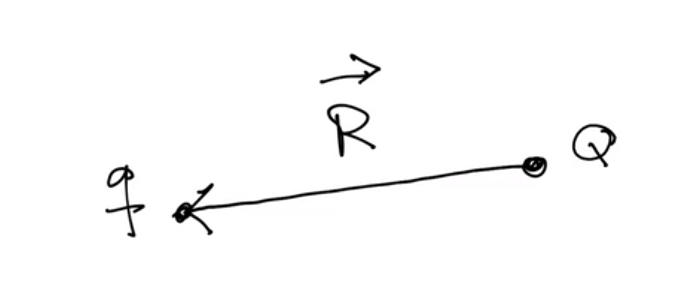
\includegraphics[scale = .7]{Bilder/Coulombs_lov.png}
      \caption{To ladde partikkler}
      \label{fig: Ladde partikkler}
    \end{figure}
  Ladning er en bevart størrelse og vil være konstant i et lukket system. \newline 

  \bf  Questions: The net force on a system due to all the electrostatic forces between charges in the system is zero. Is this statement true or false? Explain your answer. \newline \newline  
  
  \bf{True}: Kreftene vil kansellere hverandre i et større system selvom vi kan oppleve krefter lokalt. 
  
  \newpage 
  \subsection*{Eksempel}
    La oss regne ut kraften som virker på en ladning $ q $ av to andre ladninger $ Q_1, Q_2 $.
    
    \begin{figure}[ht!]
      \centering
      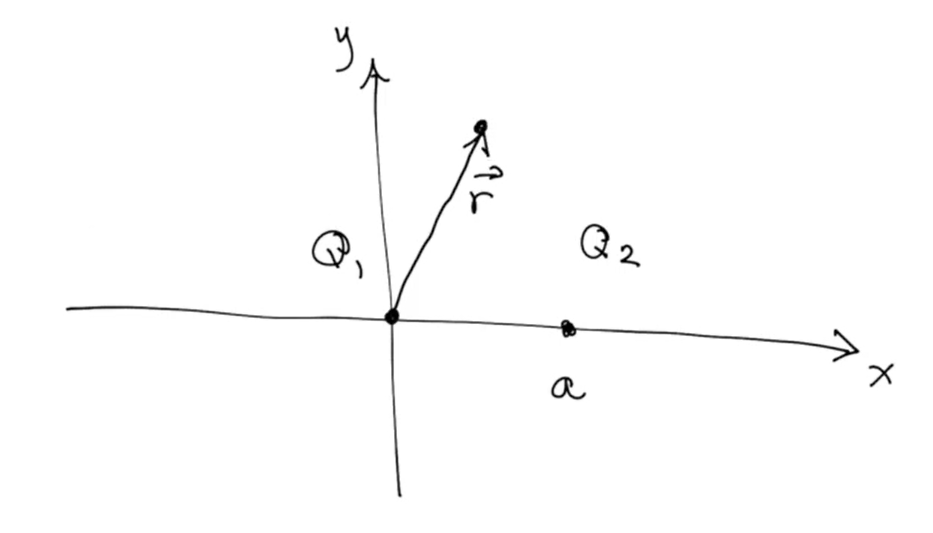
\includegraphics[scale = .7]{Bilder/Eksempel_Krefter_paa_ladning.png}
      \caption{Eksempel oppgave 1}
      \label{fig:EksempelOppgave1}
    \end{figure}
  
  Vi starter med å regne ut kraften som virker på $ q $ fra $ Q_1 $ via Coulombs lov.
  \[
  \vec{F} = \frac{qQ }{4 π \epsilon_0} \frac{\hat{R}}{R^{2}} = \frac{qQ }{4 π \epsilon_0} \frac{\vec{R}}{R^{3}}, \qquad \vec{R} = r - r_{Q_{1}} =   \begin{pmatrix}
       0  \\ 
       0 
    \end{pmatrix} - 
      \begin{pmatrix}
         a  \\ 
         0 
      \end{pmatrix} = 
  - a \hat{x}
  \]
    
  \[
  \vec{F} = \frac{qQ_1 }{4 π \epsilon_0} \frac{\vec{R}}{R^{3}} = \frac{qQ_1 }{4 π \epsilon_0} \frac{- \hat{x}}{a^{2}}
  \]
  Ettersom begge partikler har samme ladning gir det mening at kraften har en avstøtende effekt. Det eneste som skiller $ Q_1 $ og $ Q_2 $ er fortegnet på x-koordinatet. Da blir alt likt utenom $ \vec{R} $.
  \[
  \vec{F} = \frac{qQ_2 }{4 π \epsilon_0} \frac{\vec{R}}{R^{3}}, \qquad \vec{R} = \vec{r} - \vec{r}_{Q_2} = 
    \begin{pmatrix}
       a  \\ 
       0 
    \end{pmatrix} = a \hat{x}
  \]
  \[
  \vec{F} = \frac{qQ_2 }{4 π \epsilon_0} \frac{a \hat{x}}{a^{3}} = \frac{qQ_2 }{4 π \epsilon_0} \frac{\hat{x}}{a^{2}}
  \]
  \newpage
  \section*{Elektrisk felt}
  Et elektrisk felt er summen av kreftene mellom alle ladningene i et system delt på ladning til punktet vi måler fra. 
  \begin{figure}[h!]
    \centering
    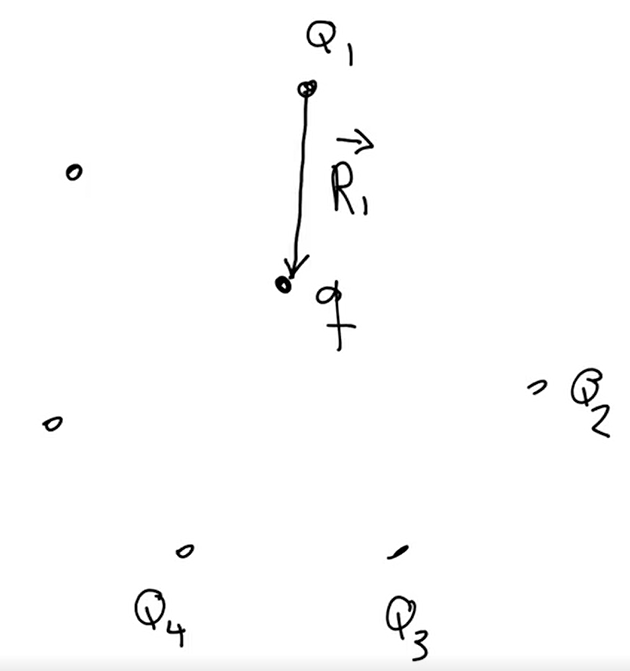
\includegraphics[scale = .7]{Bilder/Ladninger_i_felt.png}
    \caption{Illustrasjon: Ladninger i felt}
    \label{fig:Ladninger i felt}
  \end{figure}
  \[
  ∑ \limits_{}^{} \vec{F} = \frac{qQ_i }{4 π \epsilon_0} \frac{\hat{R}}{R^{2}} = q ∑ \limits_{}^{} \frac{Q_i }{4 π \epsilon_0} \frac{\hat{R}}{R^{2}}
  \]
  Alt innenfor summetegnet er definert som det elektriske feltet. 
  \[
  \vec{E} = \frac{\vec{F}}{q} = ∑ \limits_{}^{} \frac{Q_i }{4 π \epsilon_0} \frac{\vec{r} - \vec{r_i}}{\left|\vec{r} - \vec{r_i}\right| ^{3}}
  \]
  Dette gir oss det elektriske feltet i et punkt. Det betyr at feltet er avhengig av posisjonen vår $ \vec{r} $ og vi skriver det elektriske feltet som $ \vec{E}(r) $. For å finne det totalet feltet må vi summere alle feltene til alle ladningene
  \[
  \vec{E} =∑ \limits_{i}^{} \vec{E_i}
  \]
  \newpage 
  \subsection*{Eksempel }
    La oss finne det elektriske feltet med to ladninger i et vilkårlig punkt $ r $
    \begin{figure}[h!]
      \centering
      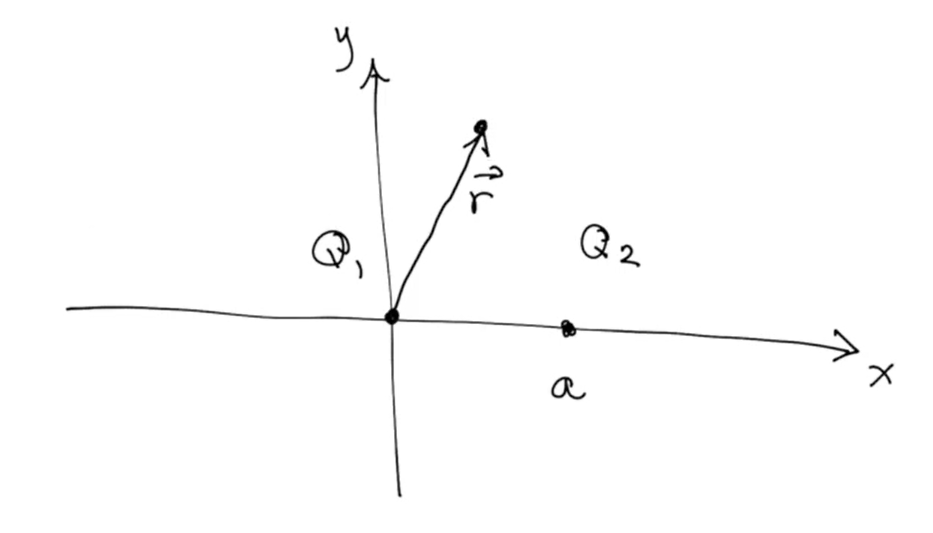
\includegraphics[scale = .7]{Bilder/Eksempel_Krefter_paa_ladning.png}
      \caption{Eksempel oppgave 2}
      \label{fig:EksempelOppgave2}
    \end{figure}
  \[
  \vec{E} = ∑ \limits_{i}^{} \frac{Q_i }{4 π \epsilon_0} \frac{\hat{R_i}}{R_i^{2}} = \frac{Q_1 }{4 π \epsilon_0} \frac{\hat{R_1}}{R_1^{2}} + \frac{Q_2 }{4 π \epsilon_0} \frac{\hat{R_2}}{R_2^{2}}, \qquad \vec{R_1} = \vec{r} - \vec{r_1} = \vec{r}, \quad \vec{R_2} = \vec{r} - \vec{r_2} = \vec{r} - (a,0)
  \]
  \[
  \vec{E} = \frac{Q_1 }{4 π \epsilon_0} \frac{\vec{r}}{r^{2}} + \frac{Q_2 }{4 π \epsilon_0} \frac{\vec{r} - a \hat{x}}{\left|\vec{r} - a \hat{x}\right|^{3}}
  \]

  \subsection*{Dipol}
    Det elektriske feltet i en dipol består av to like store, men motsatte ladninger. Vi starter med oppførselen i én dimensjon for et vilkårlig punkt langs x-aksen.
    \begin{figure}[h!]
      \centering
      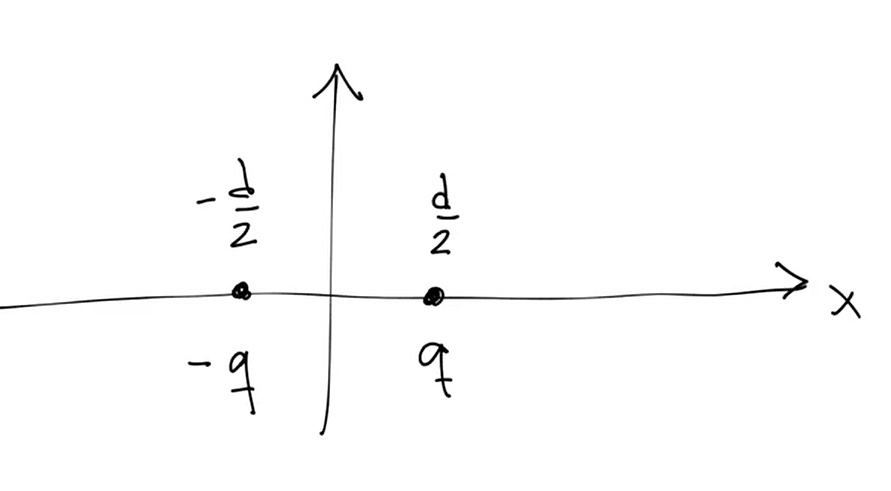
\includegraphics[scale = .4]{Bilder/Eksempel_Dipol.png}
      \caption{Eksempeloppgave: Dipol }
      \label{fig:EksempelOppgave3}
    \end{figure}

    \[
    \vec{E} =  ∑ \limits_{}^{} \frac{Q_i }{4 π \epsilon_0} \frac{\vec{R_i}}{R_i^{3}}, \qquad \vec{R_i} = \vec{r} - \vec{r_i}
    \]

    \[
    \vec{E} = \frac{1}{4 π \epsilon_0} \Bigg[ q \frac{(x,0,0) - \left(\frac{d}{2}, 0, 0\right)_{}^{}}{\left|x - \left(\frac{d}{2}\right)_{}^{}\right|^{3}} + (-q) \frac{(x,0,0) - \left(- \frac{d}{2}, 0, 0\right)_{}^{}}{\left|x + \left(\frac{d}{2}\right)_{}^{}\right|^{3}} \Bigg]_{}^{}
    \]

    \[
    \frac{q}{4 π \epsilon_0} \left[ \frac{\left(x - \frac{d}{2}\right)_{}^{}\hat{x}}{\left|x - \left(\frac{d}{2}\right)_{}^{}\right|^{3}} - \frac{\left(x + \frac{d}{2}\right)_{}^{}\hat{x}}{\left|x + \frac{d}{2}\right|^{3}} \right]_{}^{}
    \]

   En ting som er verdt å merke seg er at når $ x > \frac{d}{2} $ vil den dominere nevneren og svaret vi får vil veldig raskt bli veldig mye mindre

  \section*{Kontinuerlige ladningsfordelinger }
    Frem til nå har vi beskrevet systemene som en gruppe enkeltladninger som befinner seg i spesifikke punkter. Nå skal vi se på et område av uniformt fordelt ladning. Hvis en ser for seg at istedet for å regne ut for hver enkelt ladning, antar vi at ladningene ligger så tett inntill hverandre at vi kan bare se på det som er lite område, eller boks, med ladning. Da skriver vi om formelen for feltet slik:
    \begin{figure}[h!]
      \centering
      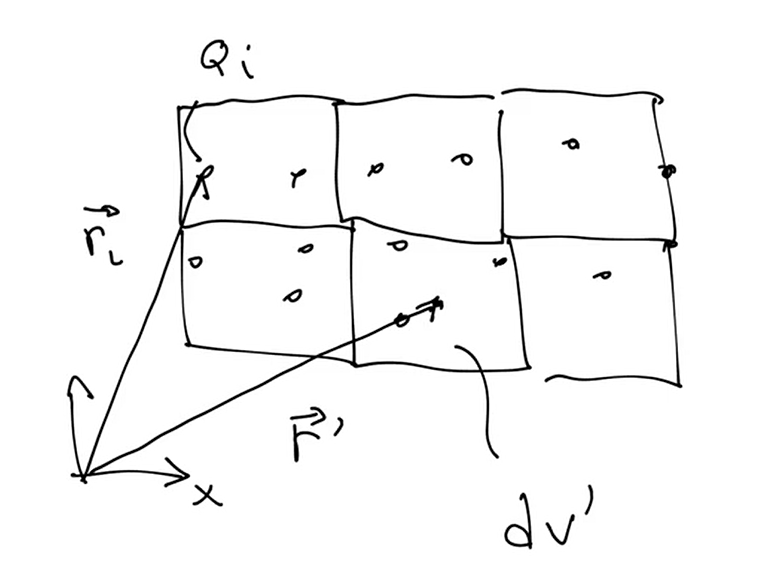
\includegraphics[scale = .7]{Bilder/Kontinuerlige_ladningsfordelinger.png}
      \caption{Kontinuerlige ladningsfordelinger }
      \label{fig:Kontinuerlige Ladningsfordelinger}
    \end{figure}

    \[
    \vec{E} = ∑ \limits_{j}^{} \frac{\Delta Q_j }{4 π \epsilon_0} \frac{\hat{R'}}{R'^{2}} = ∑ \limits_{j}^{} \frac{\Delta Q_j}{\Delta V_j} \frac{\Delta V_j }{4 π \epsilon_0} \frac{\hat{R'}}{R'^{2}}
    \]
    En kan tenke på $ \frac{\Delta Q_j}{\Delta V_j} $ som en annen måte å beskrive tetthet $ ρ(\vec{r'}) $. Når volumet blir lite nok kan dette skrives som et integral. 

    \[
    ∫_{V}^{} \frac{ρ(\vec{r'}) }{4 π \epsilon_0} \frac{\hat{R'}}{R'^{2}}\ dV' = ∫_{}^{} dq = Q
    \]
    \begin{figure}[h!]
      \centering
      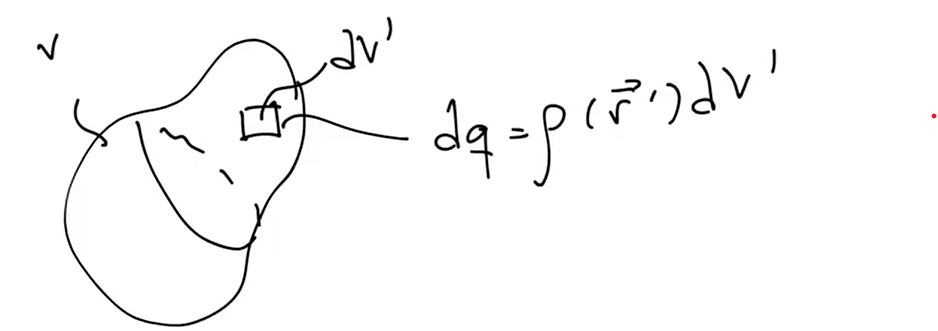
\includegraphics[scale = .7]{Bilder/3D_Ladningstetthet.png}
      \caption{Ladningstetthet i tre dimensjoner }
      \label{fig: 3DLadningstetthet }
    \end{figure}
    Dette er et tredimensjonelt eksempel. Dette kan også gjøre i to dimensjoner for en flate eller én dimensjon for en linje. 
    \begin{figure}[h!]
      \centering
      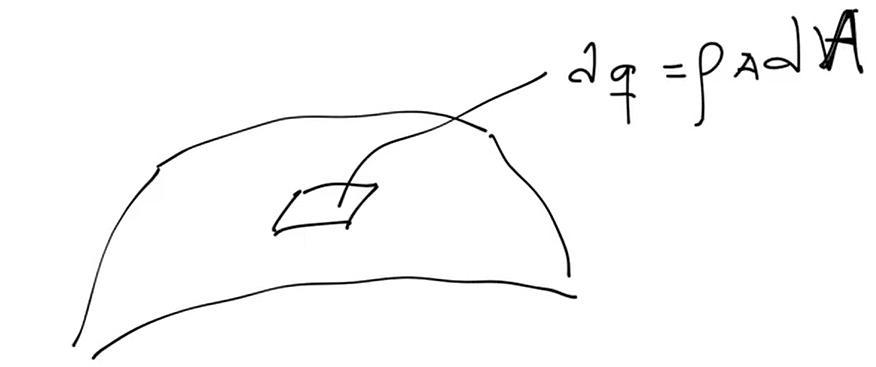
\includegraphics[scale = .6]{Bilder/2D_Ladningstetthet.png}
      \caption{Ladningstetthet i to dimensjoner}
      \label{fig: 2DLadningstetthet}
    \end{figure}

    \[
    Q = ∫_{A}^{} ρ(\vec{r'}) \ dA
    \]

    \begin{figure}[h!]
      \centering
      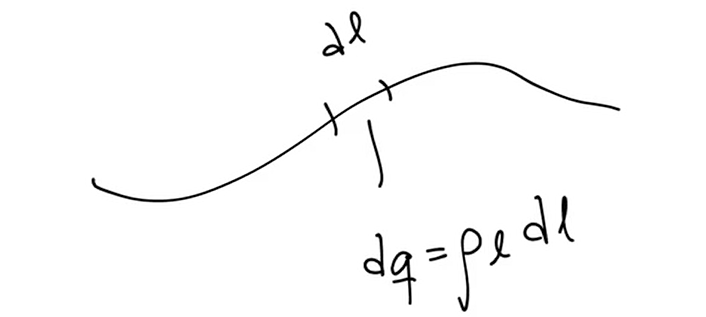
\includegraphics[scale = .6]{Bilder/1D_Ladningstetthet.png}
      \caption{Ladningstetthet i én dimensjon}
      \label{fig: 1DLadningstetthet }
    \end{figure}
    \[
    Q = ∫_{}^{} ρ e\ dl
    \]

  \subsection*{Oppgave}
    Det er en uniform ladningsfordeling $ ρ $ i område $ 0<x<a, 0<y<b, 0<z<c $. Hva blir integralet? \newline 

  





